\newpage
\section{DSL - System Details}

\subsection{Architecture of System}

The diagram below describes the architecture of the system.

\begin{figure}[H]
  \centering
    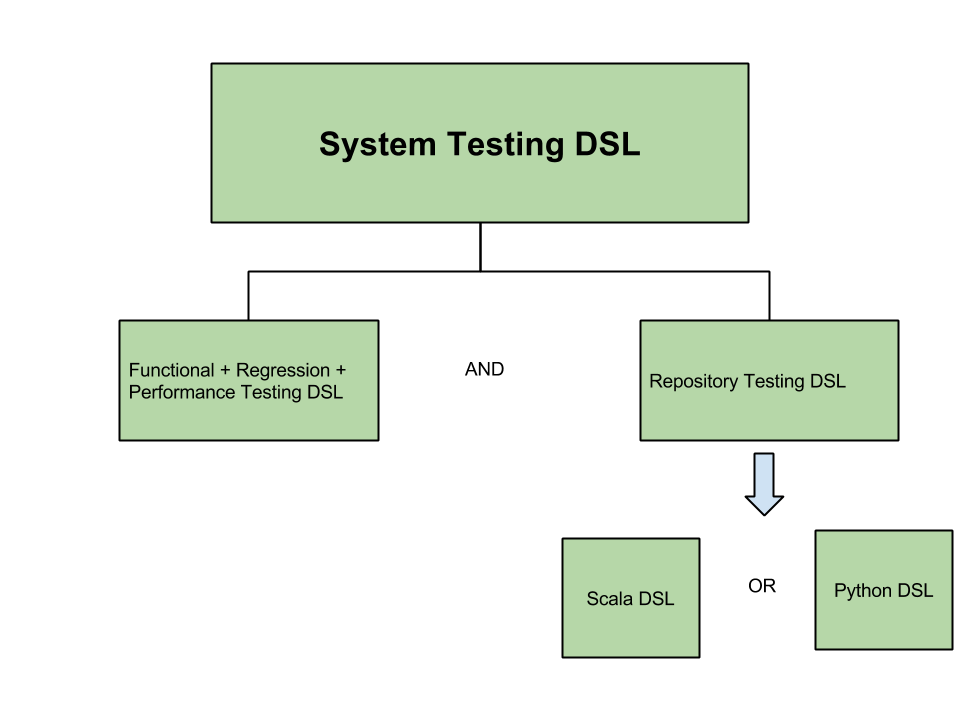
\includegraphics[width=450px]{figures/architecture.png}
  \caption{Architecture of System Testing DSL}
\end{figure}

\noindent
The system testing DSL comprises two DSLs that are composed with one other:
\begin{itemize}
\item DSL for regression, functional and performance testing
\item DSL for repository testing
\end{itemize}

\noindent
The composition of both DSLs to achieve system testing is shown below in a diagram:

\begin{figure}[H]
  \centering
    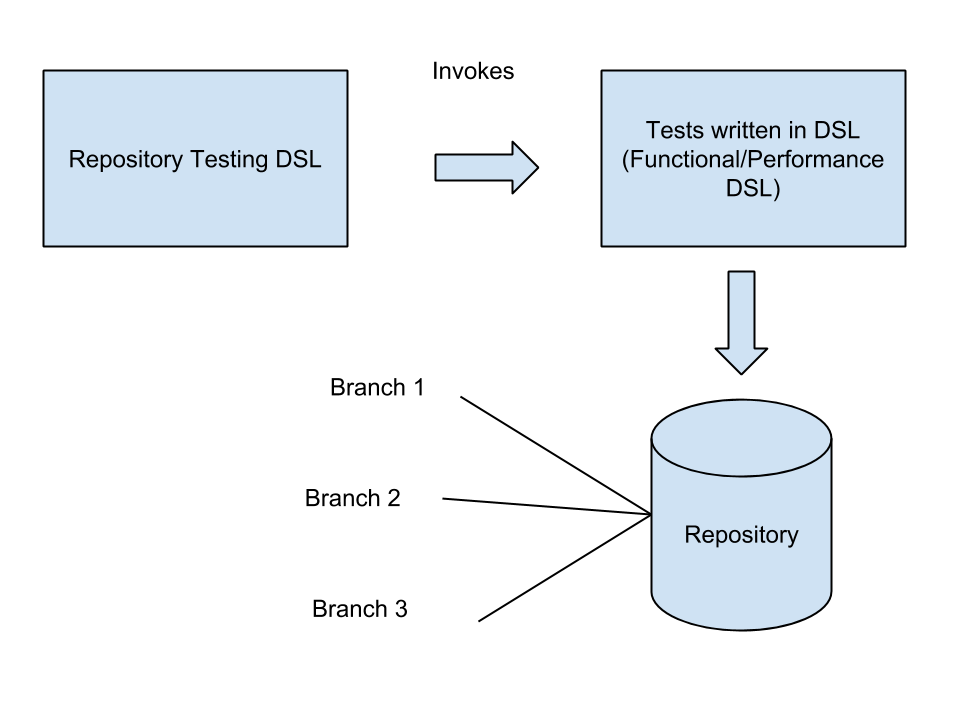
\includegraphics[width=450px]{figures/repo_test_diagram.png}
    \caption{Composition Repository Testing and Functional/Performance Testing DSL}
\end{figure}

\noindent
Two versions of the repository testing DSL were developed. The first version was developed in the dynamic language - Python and the second one was developed in Scala. This was done to compare the two DSLs developed on the basis of development times, type safety, syntax and usability.

\subsection{DSL in Scala for Functional, Regression and Performance Testing}
The first DSL performs regression testing, performance testing and functional testing.

\subsubsection{Regression Testing}
\textbf{Regression Testing} is one of the key features of the DSL. Users can generate \textbf{reference tests} with a certain ideal set of data and then run tests against the \textbf{regression reference} conveniently. All the test specific details can be configured using a configuration file - \textbf{application.conf}. The configuration file is written in YAML markup but stored with the extension .conf as the Scala configuration library developed by Typesafe implicitly loads .conf files.
\bigskip

\noindent
The markup approach allows users to write regression tests \textit{without} writing any code and just specifying certain settings in plain text. This adds to meaning to the domain models developed and gives the DSL a declarative feel.

\bigskip
\begin{figure}[H]
  \centering
    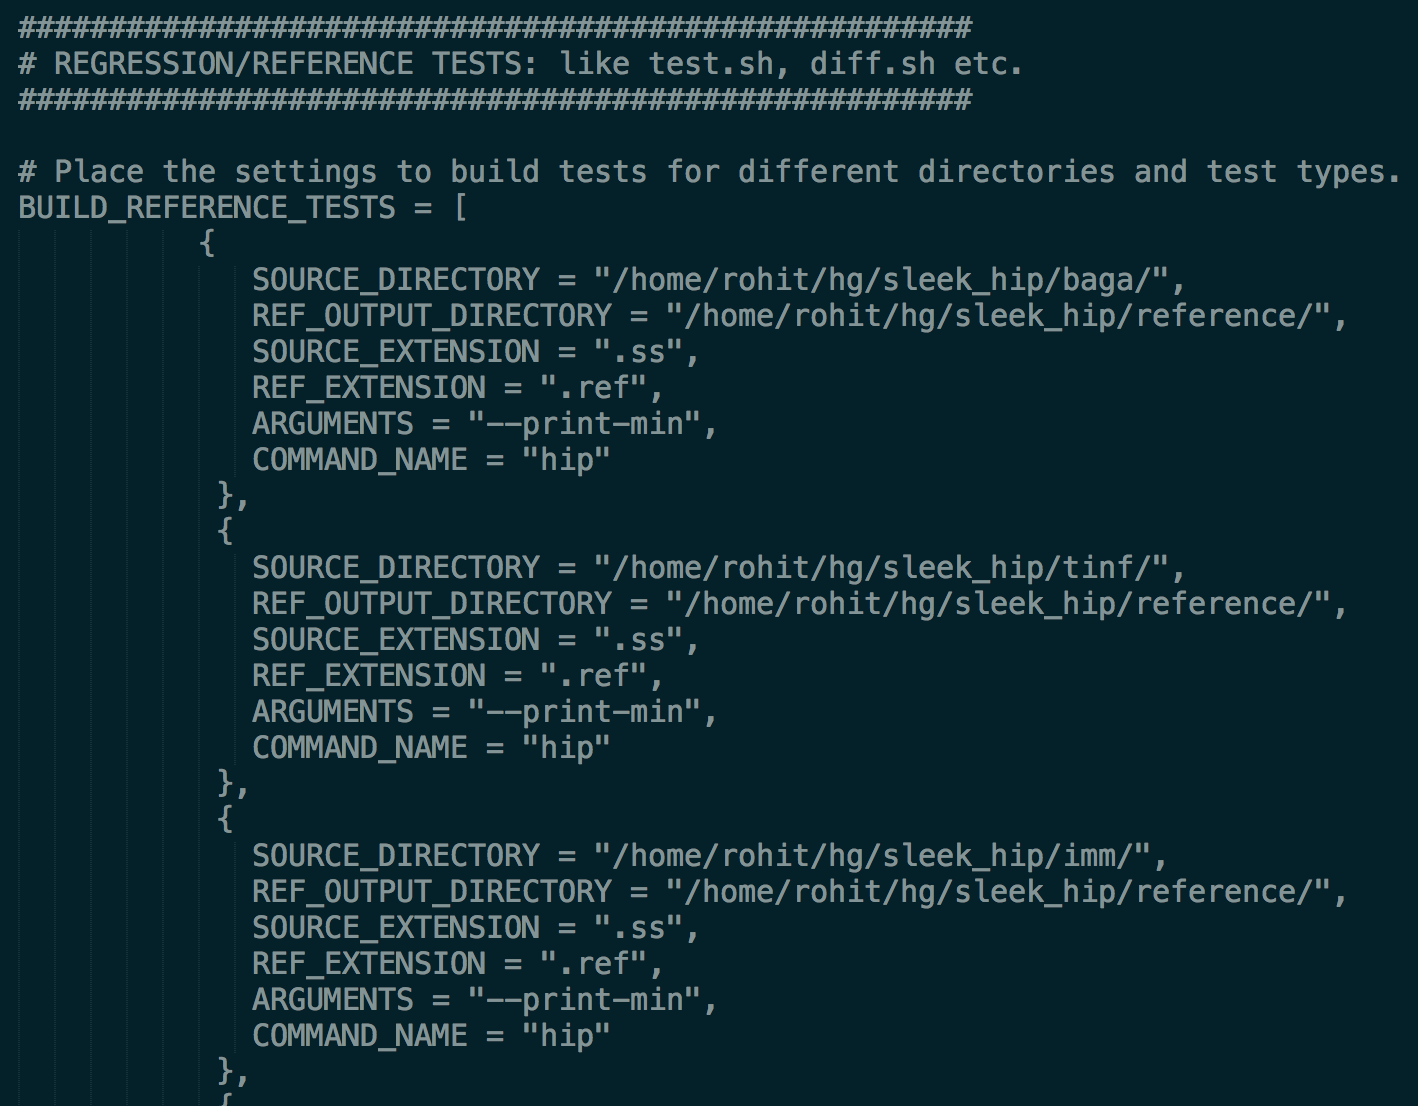
\includegraphics[height=250px]{figures/application_conf.png}
  \caption{application.conf - the driver for regression tests}
\end{figure}

\noindent
For regression testing there are 3 primary options provided  - \textbf{buildReference, runReference and overrideReference}. The first one creates a repository of reference results for specified tests. The second option runs a set of tests against the stored references. The last option is for selectively rebuilding reference results. For example, a certain test in a test suite may have changed so it's reference result has to be changed.
\bigskip

\begin{figure}[H]
  \centering
    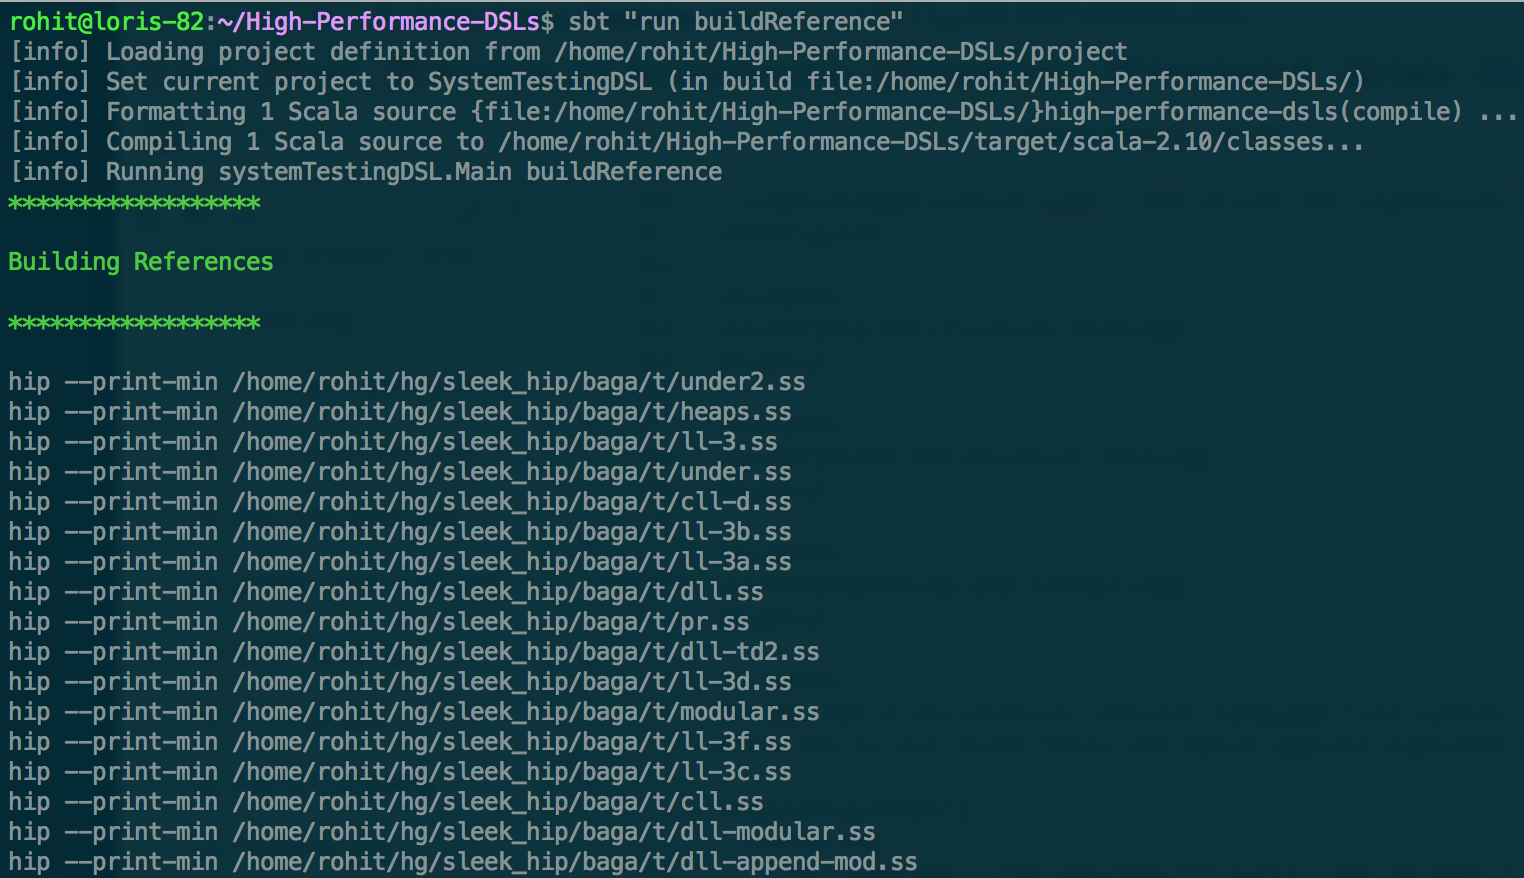
\includegraphics[height=300px]{figures/building_reference.png}
  \caption{Building References for Regression Testing}
\end{figure}

\subsubsection{Functional Testing}
\textbf{Hip Verification Testing} was one of the first applications of the DSL. The \textbf{HIP/SLEEK} systems are aimed at automatic verification of functional correctness of heap manipulating programs. HIP is a separation logic based automated verification system for a simple imperative language, able to modularly verify the specifications of heap-manipulating programs \cite{hipsleek}. The DSL developed can perform HIP lemma testing. Running with the option \textbf{"hip"} tests the hip files. The screen - shot below shows the hip tests running. Coloured console output showing outcome is shown.
\bigskip

\begin{figure}[H]
  \centering
    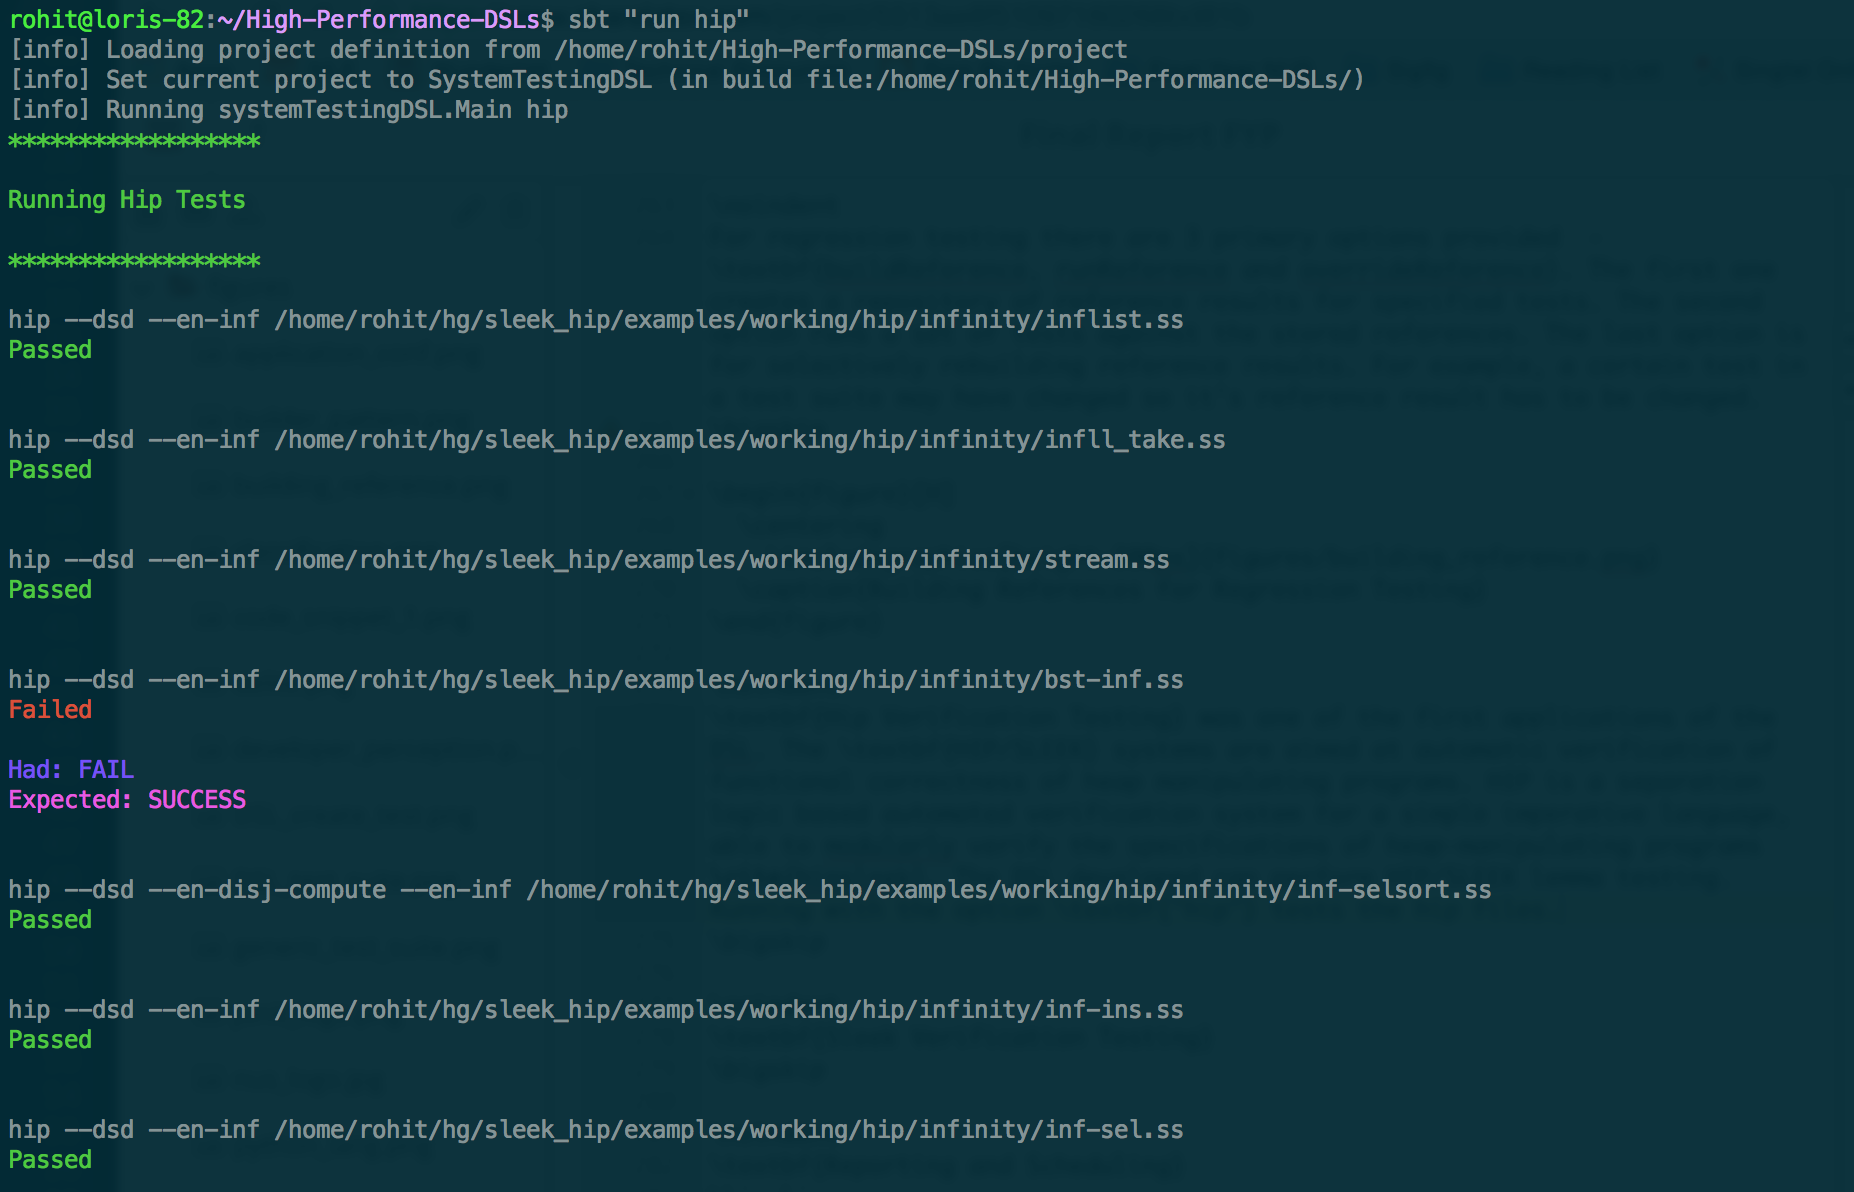
\includegraphics[height=320px]{figures/hip_testing.png}
  \caption{Running Hip Tests}
\end{figure}

\noindent
\textbf{Sleek Verification Testing} is also one of the main applications of the DSL currently. The various Sleek Entails can be verified by running the \textbf{sleek} option in the DSL. The DSL uses specific \textbf{regular expressions} and \textbf{parsing rules} to ascertain whether an entail has been correctly passed or failed. The DSL provides extensibility in terms of output produced. It has \textbf{Console output} and \textbf{HTML output} capabilities allowing the system to produce \textbf{browser - friendly content}.
\bigskip

\begin{figure}[H]
  \centering
    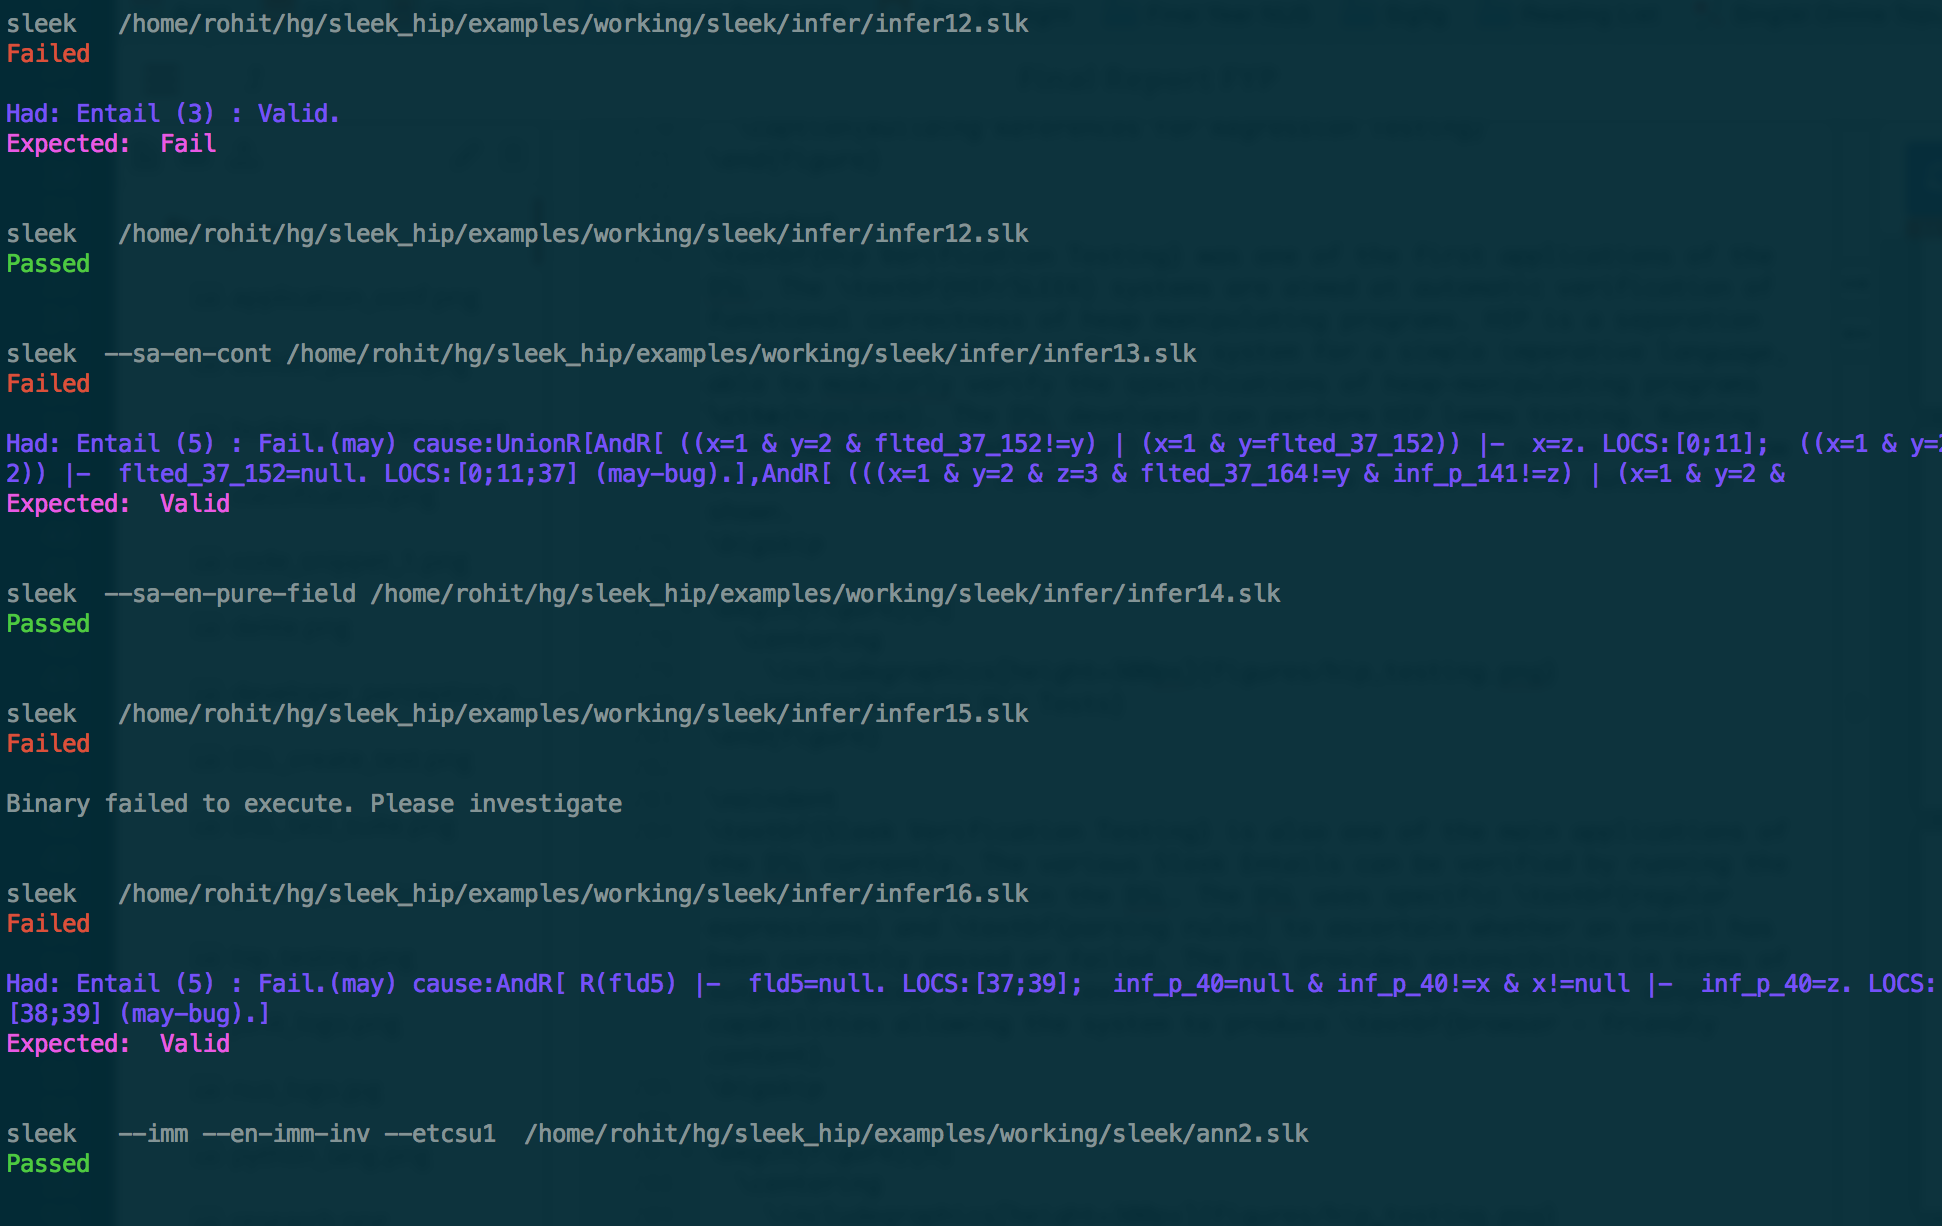
\includegraphics[height=300px]{figures/sleek_testing.png}
  \caption{Running Sleek Tests Console Output}
\end{figure}

\begin{figure}[H]
  \centering
    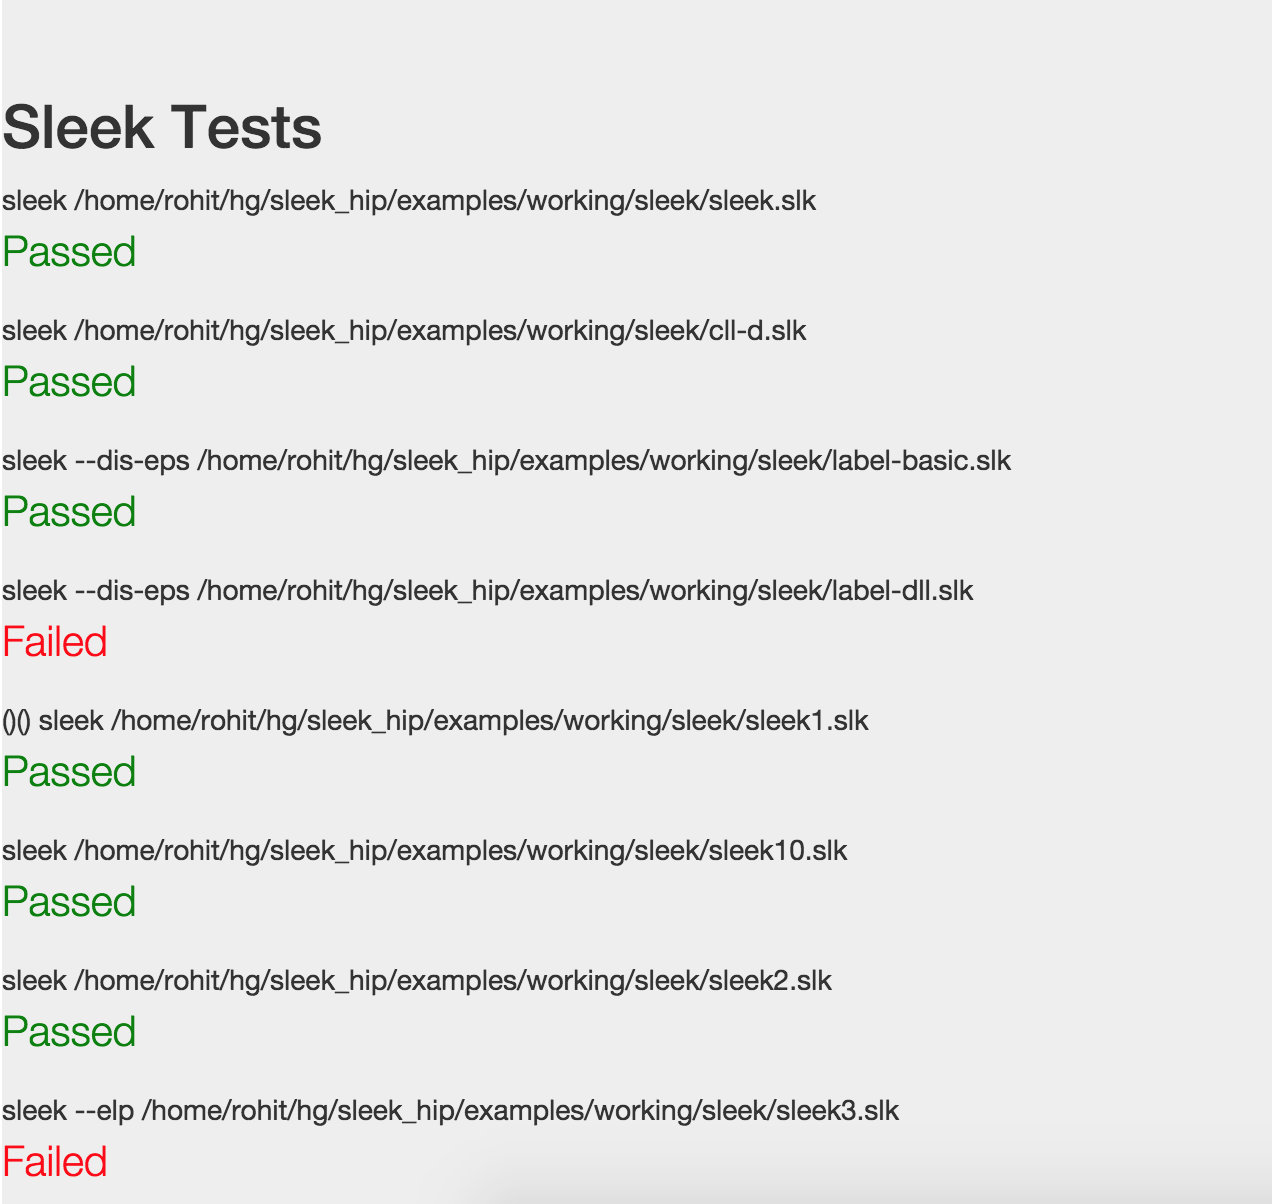
\includegraphics[height=350px]{figures/web_output_1.png}
  \caption{Running Sleek Tests HTML Output}
\end{figure}

\noindent
After running all the tests, \textbf{test statistics} are produced in addition to \textbf{logged output}. \textbf{JUnit} was the inspiration for such a command line interface.

\begin{figure}[H]
  \centering
    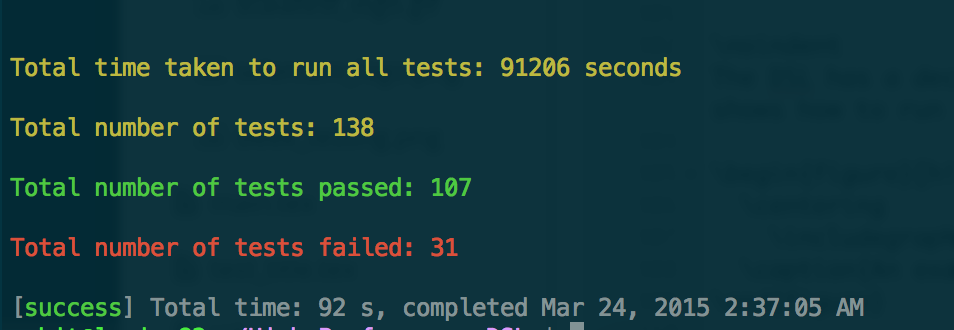
\includegraphics[height=150px]{figures/test_statistics.png}
  \caption{Test statistics at the end of every test Console Output}
\end{figure}

\begin{figure}[H]
  \centering
    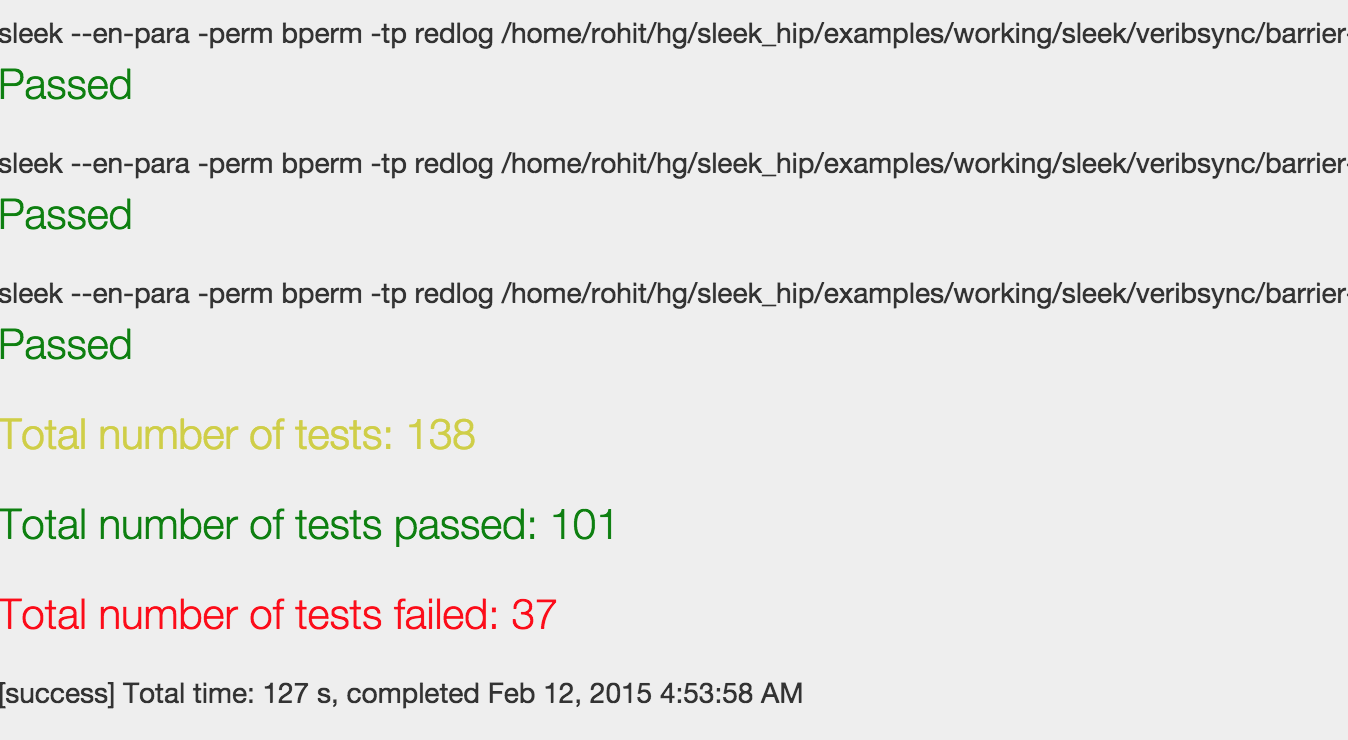
\includegraphics[height=220px]{figures/web_output_2.png}
  \caption{Test statistics at the end of every test HTML Output}
\end{figure}

\noindent
The figure above shows the test statistics screen being rendered for browser - friendly viewing (in HTML). 

\subsubsection{Performance Testing}

The DSL supports performance testing and generates reports to \textit{HTML} or \textit{Console} with a description of tests that overran the expected duration with their respective file names. This helps developers quickly inspect failing performance tests. A screen - shot of the performance report is shown below:

\begin{figure}[H]
  \centering
    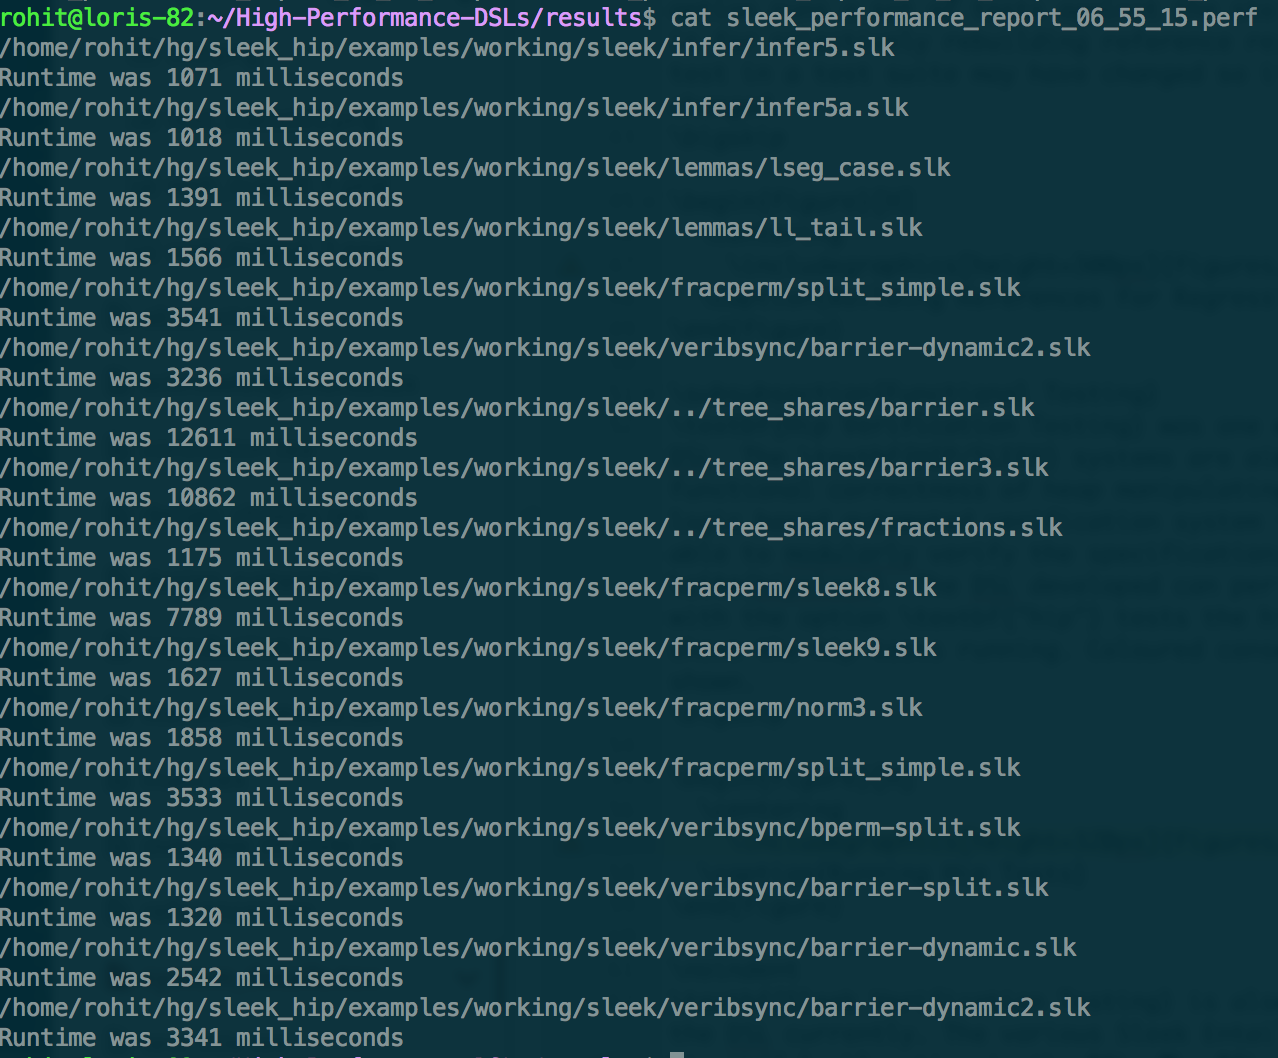
\includegraphics[width=300px]{figures/performance_testing.png}
  \caption{Performance Report for Sleek Tests}
\end{figure}

\noindent
The threshold value for performance tests can be specified in the YAML file \textit{application.conf}

\subsection{DSL in Scala and Python for Repository Testing}

\noindent
\textbf{Repository Testing} has been decoupled from the core DSL and are written in a separate DSL. \textbf{Two} versions of this DSL were written - one in \textbf{Python} and the other in \textbf{Scala}. This was done to understand the difference in constructing DSLs in a dynamic language like Python as opposed to a static typed language like Scala. Some of the features of this DSL are: 
\begin{itemize}
\item Check out different branches of a mercurial repository
\item Run the DSL's tests (functional/performance/regression) against each branch
\item Summarize the results conveniently in a hierarchical directory
structure
\item Run tests against each commit as long as it is a new commit (users can define what they mean by "new" using a \textbf{settings.yaml } file)
\end{itemize}

\begin{figure}[H]
  \centering
    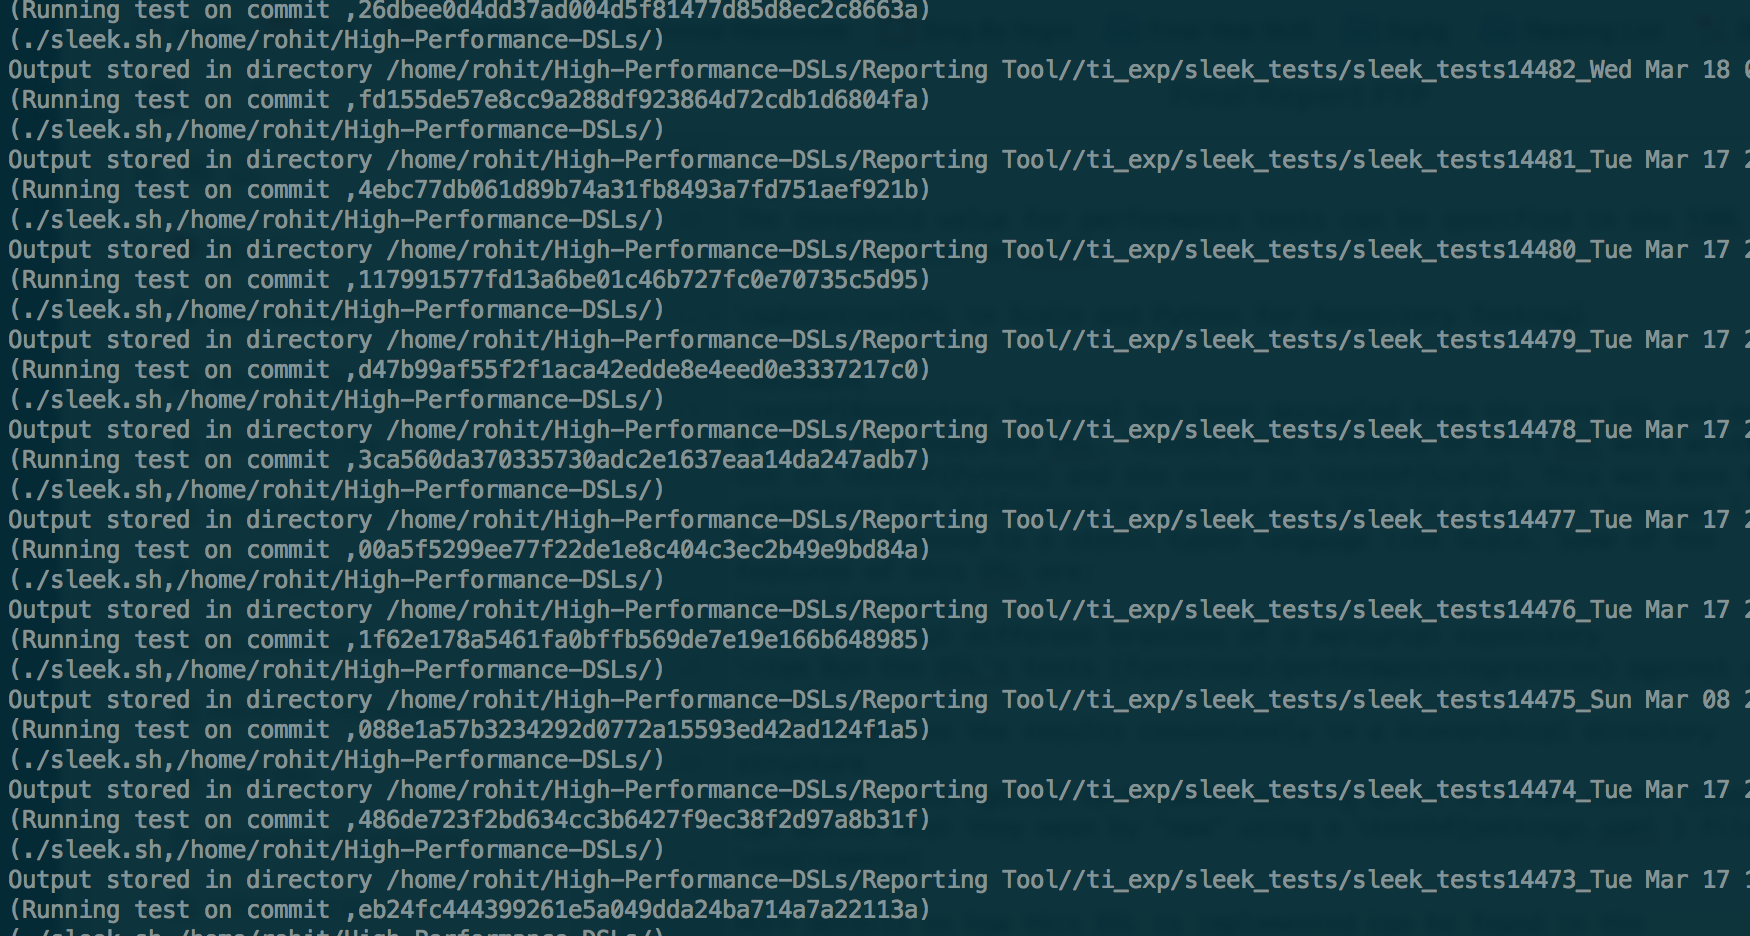
\includegraphics[width=500px]{figures/repo_testing.png}
  \caption{Repository level tests being run on the HIP/SLEEK code base}
\end{figure}

\noindent
In the screen - shot above, the DSL is checking out different commits on different branches within the last 100 days and running functional and performance tests against each of these branches/commits. The \textit{repository testing DSL} invokes necessary methods in the first DSL to run these tests. More details on how this DSL is implemented can be found in the \textbf{Design Choices} section.
\bigskip

\newpage
\subsection{Software Engineering Methodology}

The project was built over the period of one year following certain software engineering methodologies. Some of these methodologies are:
\begin{itemize}
\item \textbf{Test Driven Development (TDD)}: Test-driven development (TDD) is a software development process that relies on the repetition of a very short development cycle: first the developer writes an (initially failing) automated test case that defines a desired improvement or new function, then produces the minimum amount of code to pass that test \cite{tdd}. Tests for the DSL can be found in \textbf{src/test/scala/systemTestingDSL/} and can be executed by running \textbf{"sbt test"}.

\begin{figure}[H]
  \centering
    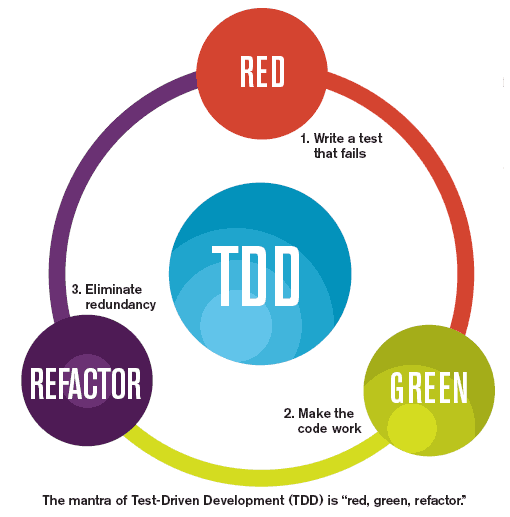
\includegraphics[height=130px]{figures/tdd.png}
%   \caption{}
\end{figure}

\item \textbf{Agile Software Development}: Agile development provides opportunities to assess the direction throughout the development life - cycle. Every few days (in this case 2 weeks), new features are shown to the users and based on feedback and criticism from them, changes are made. This process is continued throughout the entire life - cycle of the project ]\cite{agile}.

\begin{figure}[H]
  \centering
    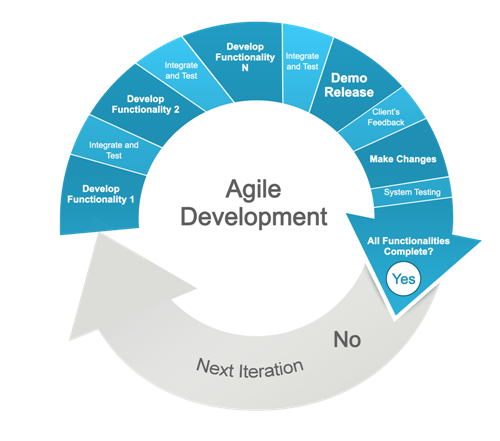
\includegraphics[height=150px]{figures/agile.png}
  \caption{Agile explained}
\end{figure}
\end{itemize}

\newpage